\documentclass[12pt, a4paper]{article}

\usepackage{tikz}

\usetikzlibrary{automata,positioning}

% \usepackage{syntax}
% \usepackage{etoolbox}
% \AtBeginEnvironment{tikzpicture}{\catcode`\_=8}

\title{Graphs and automata}
\author{wye}

\begin{document}
\maketitle
\newpage

    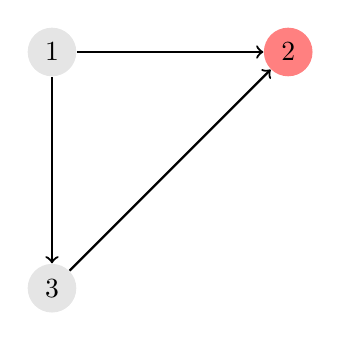
\begin{tikzpicture}
        \tikzstyle{vertex} = [circle, fill=black!10]
        \tikzstyle{selected vertex} = [vertex, fill=red!50]
        \tikzstyle{edge} = [->, thick]

        \node[vertex](v1) at(0, 0) {1};
        \node[selected vertex](v2) at(3, 0) {2};
        \node[vertex](v3) at(0, -3) {3};

        \draw[edge] (v1) -- (v2);
        \draw[edge] (v1) -- (v3);
        \draw[edge] (v3) -- (v2);
    \end{tikzpicture}

    \vspace{20pt}
    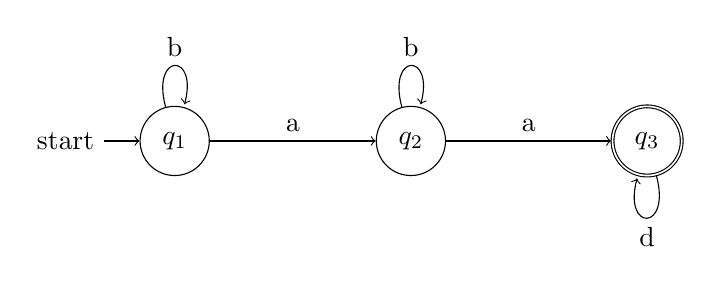
\begin{tikzpicture}[->, node distance=3cm, auto]
        \node[initial, state] (A) {$q_1$};
        \node[state] (B) [right of=A] {$q_2$};
        \node[state, accepting] (C) [right of=B] {$q_3$};

        \path (A) edge [loop above] node {b} (A)
              edge node {a} (B)
              (B) edge [loop above] node {b} (B)
              edge node {a} (C)
              (C) edge [loop below] node {d} (C)
        ;
    \end{tikzpicture}

    \vspace*{20pt}

    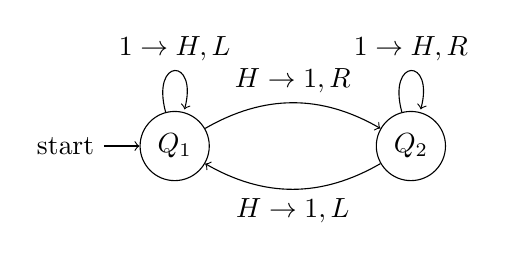
\begin{tikzpicture}[->, node distance=3cm, auto]
        \node[initial, state] (A) {$Q_1$};
        \node[state] (B) [right of=A]{$Q_2$};

        \path (A) edge[loop above] node {$1 \rightarrow H,L$} (A)
              edge[bend left] node {$H \rightarrow 1,R$} (B)
              (B) edge[bend left] node {$H\rightarrow 1,L$} (A)
              edge[loop above] node {$1 \rightarrow H,R$} (B)
        ;        
    \end{tikzpicture}
    \vspace*{20pt}

    \begin{tikzpicture}[->, node distance=3cm, auto]
        \node[initial, state] (A) {};
        \node[state] (B)[right of=A] {};
        \node[state] (C)[below of=A] {};
        \node[sttex_exer/dataflow/automata.texate] (D)[right of=C] {};
        \node[state] (E)[right of=D] {};

        \path (A) edge[bend left] (B)
              edge (B)
              (B) edge[bend left] (A)
              edge (D)
              (C) edge (A)
                  edge[loop below] (C)
              (D) edge (C)
                  edge (E)
        ;
    \end{tikzpicture}
\end{document}